\documentclass{report}
\usepackage{graphicx}

\usepackage{amsmath}
\DeclareMathOperator*{\argmax}{argmax}

\usepackage{hyperref}
\hypersetup{
    colorlinks=true,
    linkcolor=blue,
    filecolor=magenta,      
    urlcolor=cyan,
}

\begin{document}

\title{Banana World Project Report}
\author{Denis Sergeev}


\section*{Problem definition}

The goal of the project was to create a RL Agent which is able to train from scratch by interacting with the Reacher (robot arm) environment for a series of episodes. During the episode the agent receives the environment state. The agent is able to perform some actions which may change the environment state.

\subsection*{Environment description}

In this environment, a double-jointed arm can move to target locations. A reward of \(+0.1\) is provided for each step that the agent's hand is in the goal location. Thus, the goal of the agent is to maintain its position at the target location for as many time steps as possible.

The observation space consists of 33 variables corresponding to position, rotation, velocity, and angular velocities of the arm. Each action is a vector with four numbers, corresponding to torque applicable to two joints. Every entry in the action vector should be a number between \(-1\) and \(1\).

The barrier for solving the problem is that all agents must get an average score of +30 (over 100 consecutive episodes). Specifically, after each episode, we add up the rewards that each agent received (without discounting), to get a score for each agent. This yields 20 (potentially different) scores. We then take the average of these 20 scores. This yields an average score for each episode (where the average is over all 20 agents).


\section*{Solution}
\subsection*{Deep Deterministic Policy Gradient Algorithm}
\subsubsection*{Network}
The DDPG algorithm uses two neural networks, an actor and a critic. Each one has two copies, a local and a target one. The Actor is trained to give the best possible action, given the current state of the environment. \(s => a\). The Critic is trained to give an estimate of the reward that'd be obtained if an action A is applied at the state \(s\). \((s, a) => V\) Local networks are trained to get the "labels" given by the target.

Both networks consist of fully connected units with batch normalization and ReLu activation. The input to the actor network is the environment state, which goes through 3 fully connected layers. The final activation function is \(tanh\), since the action value should be in-between \(-1\) and \(1\).

The input to the critic is the environment state, which goes through the first fully connected layer. After batch normalization and ReLu activation it is concatenated with the action tensor and goes through the remaining 2 layers.

\subsection*{Training}
\subsubsection*{Loss function and optimizing method}

DDGP algorithm uses following loss function for critic network \ref{critic-loss}:
\begin{equation} \label{critic-loss}
L \equiv (R_t + \gamma Q(S_{t+1}, a_{t+1}; \theta'_t) - Q(S_t, a_t; \theta_t))^{2}
\end{equation}

Where \(Q(S_t, a_t; \theta_t)\) is output (value of action) of the critic network with internal parameters \(\theta_t\) given input \(S_t\) and \(a_t\). \(a_{t+1}\) is obtained from \(\pi(S_t; \eta'_t)\) (target actor) prediction with internal parameters \(\eta'_t\).

Actor loss function is following \ref{actor-loss}:
\begin{equation} \label{actor-loss}
L \equiv -(Q(S_t, \pi(S_t; \eta_t); \theta_t))
\end{equation}

Both loss functions used 2 sets of network parameters: target \(\theta'_t\), \(\eta'_t\) and local \(\theta_t\), \(\eta_t\). Target network parameters are updating through soft update \(\theta'_t = (1 - \tau) \theta'_t + \tau \theta_t\).
As optimizing method for both networks I used Adam with learning rate \(\alpha\).

\subsubsection*{Experience replay}
The input for training did not come directly from episodes. Instead I used experience replay technique (see \href{https://storage.googleapis.com/deepmind-media/dqn/DQNNaturePaper.pdf}{Human-level control through deep reinforcement learning}).

\subsubsection*{Exploratory noise}
In order to make the agent explore the environment DDPG algorithm adds noise in it actions during training. I used \href{https://en.wikipedia.org/wiki/Ornstein-Uhlenbeck_process}{Ornstein–Uhlenbeck process} for this purpose.


\section*{Results}

I came up using following training hyper parameters:
\begin{itemize}
	\item Buffer size: 10e6
	\item Batch size: 128
	\item \(\gamma\): 0.95
	\item \(\tau\): 0.001
	\item \(\alpha_{actor}\): 0.0001
	\item \(\alpha_{critic}\): 0.001
\end{itemize}
They were used across all training experiments below.


\subsection*{Training DDPG 128x256 128x256}

DDPG actor: 128x256, critic 128x(256+31).

Training history:

Episode 10.	Average Score: 1.29.	Time elapsed: 4:41

Episode 20.	Average Score: 2.01.	Time elapsed: 9:22

Episode 30.	Average Score: 3.98.	Time elapsed: 14:12

Episode 40.	Average Score: 8.78.	Time elapsed: 19:10

Episode 50.	Average Score: 13.40.	Time elapsed: 24:40

Episode 60.	Average Score: 16.83.	Time elapsed: 29:54

Episode 70.	Average Score: 19.30.	Time elapsed: 35:04

Episode 80.	Average Score: 21.39.	Time elapsed: 40:21

Episode 90.	Average Score: 22.95.	Time elapsed: 46:02

Episode 100.	Average Score: 24.32.	Time elapsed: 51:54

Episode 110.	Average Score: 27.81.	Time elapsed: 57:52

Environment solved in 17 episodes!	Average Score: 30.10.	Time elapsed: 62:04. See \ref{fig:DDPG_128x256}.

\begin{figure}
	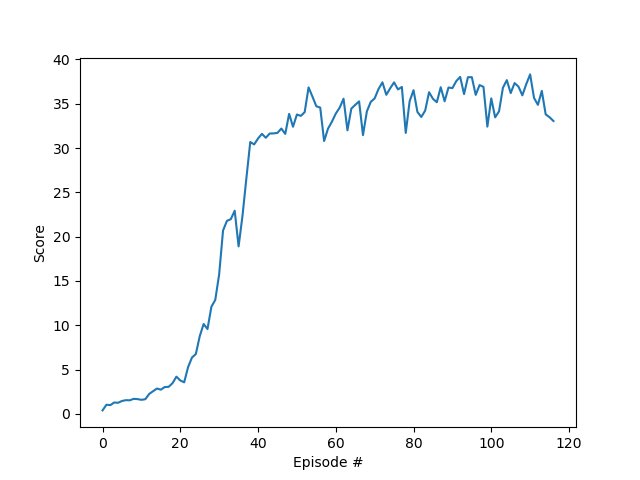
\includegraphics[width=0.9\linewidth]{res/ddpg_128x256/score.png}
	\caption{DDPG 128x256: Rewards per episode}
	\label{fig:DDPG_128x256}
\end{figure}


\subsection*{Training DDPG 128x128 128x128}

DDPG actor: 128x128, critic 128x(128+31).

Episode 10.	Average Score: 0.48.	Time elapsed: 2:00

Episode 20.	Average Score: 0.95.	Time elapsed: 4:26

Episode 30.	Average Score: 1.47.	Time elapsed: 7:16

Episode 40.	Average Score: 2.20.	Time elapsed: 10:27

Episode 50.	Average Score: 3.02.	Time elapsed: 13:59

Episode 60.	Average Score: 4.29.	Time elapsed: 17:43

Episode 70.	Average Score: 5.77.	Time elapsed: 21:24

Episode 80.	Average Score: 7.87.	Time elapsed: 25:11

Episode 90.	Average Score: 9.93.	Time elapsed: 29:02

Episode 100.	Average Score: 12.19.	Time elapsed: 33:03

Episode 110.	Average Score: 15.77.	Time elapsed: 37:09

Episode 120.	Average Score: 19.19.	Time elapsed: 41:21

Episode 130.	Average Score: 22.43.	Time elapsed: 45:05

Episode 140.	Average Score: 25.19.	Time elapsed: 48:39

Episode 150.	Average Score: 27.81.	Time elapsed: 52:17

Episode 160.	Average Score: 29.93.	Time elapsed: 56:03

Environment solved in 61 episodes!	Average Score: 30.14.	Time elapsed: 56:25. See \ref{fig:DDPG_128x128}.

\begin{figure}
	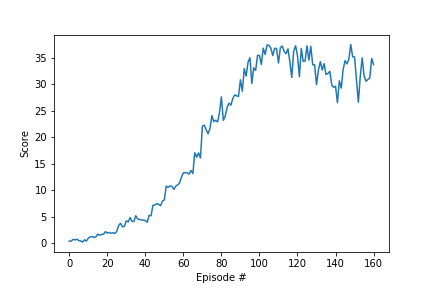
\includegraphics[width=0.9\linewidth]{res/ddpg_128x128/score.png}
	\caption{DDPG 128x128: Rewards per episode}
	\label{fig:DDPG_128x128}
\end{figure}


\subsection*{Conclusion}

From the above results we can summarize, that actor: 128x256, critic 128x(256+31) networks architecture have better performance and learn faster than actor: 128x128, critic 128x(128+31). In overall DDPG algorithm performs very good in this environment.


\section*{Areas of improvement}

I also tried to implement \href{https://arxiv.org/pdf/1707.06347.pdf}{PPO algorithm}. I used some code form \href{https://github.com/ShangtongZhang/DeepRL}{Shangtong Zhang DeepRL github repository} to build more intuition about PPO and be more confident in correct implementation. But implemented algorithm almost didn't perform. Seems like something is still wrong. PPO algorithm is said to be more stable and perform better.

Another improvement could be implementing \href{https://arxiv.org/abs/1511.05952}{prioritized experience replay} in DDPG algorithm.

\end{document}
